\normaltrue \difficilefalse \tdifficilefalse
\correctiontrue

%\UPSTIidClasse{11} % 11 sup, 12 spé
%\newcommand{\UPSTIidClasse}{11}

\exer{La Seine Musicale$\star$ \label{B2:07:39}}
\setcounter{question}{0}\marginnote{\xpComp{SLCI}{03}}%\UPSTIcompetence{B2-07}
\index{Compétence B2-07}\index{Compétence SLCI-03}
\index{La Seine Musicale}
\ifcorrection
\else
\marginnote{\textbf{Pas de corrigé pour cet exercice.}}
\fi

\ifprof
\else
Soit le schéma-blocs suivant. 
\begin{figure}[!h]
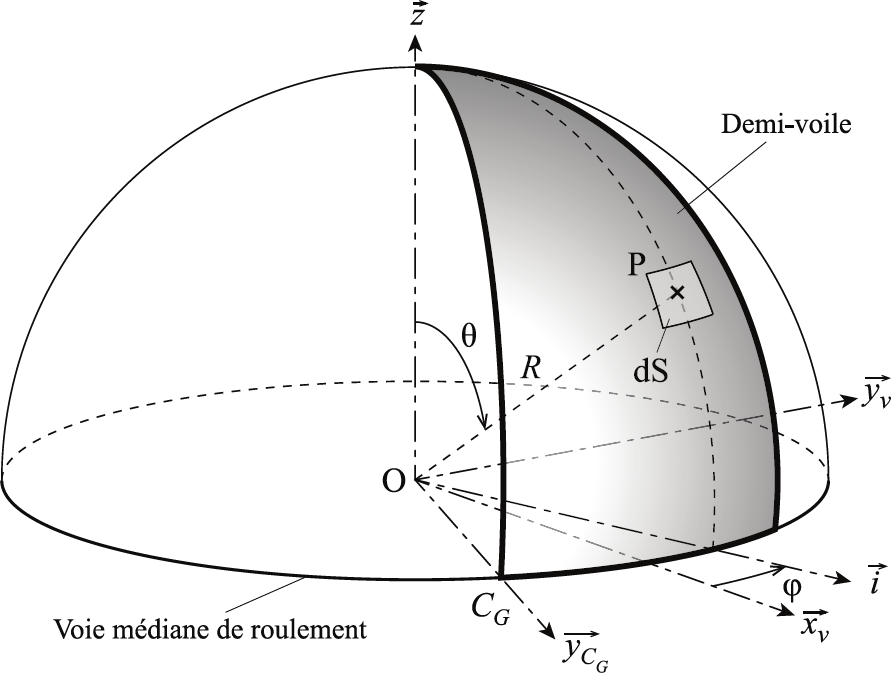
\includegraphics[width=\linewidth]{39_01}
%\caption{ \label{fig_39_01}}
\end{figure}
\fi

\question{En considérant que la perturbation $C_{\text{pert}}(p)$ est nulle, déterminer $H_f(p)=\dfrac{\Omega_m(p)}{\Omega_c(p)}$ sous forme canonique.}
\ifprof
Réduction de la boucle du moteur à courant continu : 
$\dfrac{\Omega_m(p)}{U_m(p)}=\dfrac{\dfrac{k_c}{R+Lp}\dfrac{1}{J_{eq}p}}{1+\dfrac{k_c}{R+Lp}\dfrac{k_e}{J_{eq}p}}$
$=\dfrac{k_c}{\left(R+Lp\right)J_{eq}p+k_ek_c}$.

On a alors, 

$
\dfrac{X_{ch}(p)}{\Omega_c(p)} =
K_a  \dfrac{CK_h \dfrac{k_c}{\left(R+Lp\right)J_{eq}p+k_ek_c}}{1+CK_hK_{\text{capt}} \dfrac{k_c}{\left(R+Lp\right)J_{eq}p+k_ek_c}}
$ 

$
=
K_a \dfrac{CK_h k_c}{\left(R+Lp\right)J_{eq}p+k_ek_c+CK_hK_{\text{capt}} k_c}
$

$
=
\dfrac{K_a }{\left( k_ek_c+CK_hK_{\text{capt}} k_c\right)} \dfrac{CK_h k_c}{\dfrac{J_{eq}\left(R+Lp\right)}{k_ek_c+CK_hK_{\text{capt}} k_c}p+1}
$.

\else
\fi

\question{En prenant $\Omega_c(p)=0$, exprimer la fonction de transfert $H_r(p)=\dfrac{\Omega_m(p)}{C_{\text{pert}}(p)}$ en la mettant sous la forme : $H_r(p)=-\dfrac{\alpha \left(1+\tau p\right)}{1+\gamma p+\delta p^2}$. Exprimer $\alpha$, $\tau$, $\gamma$ et $\delta$ en fonction des différents paramètres de l’étude.}
\ifprof ~\\
Par lecture directe du schéma-blocs, on a 
$\Omega_m(p) = \dfrac{1}{J_{eq}p}\left(C_{\text{pert}}(p) + C_m(p)\right)$.

De plus, 
$C_m(p) = \left(U_m(p)-k_e\Omega_m(p)\right) \dfrac{k_c}{R+Lp}$
 et $U_m(p)=\varepsilon(p) C K_h = -\Omega_m(p) C K_h K_{\text{capt}}$.
 
 On a donc, 
 
 $\Omega_m(p) = \dfrac{1}{J_{eq}p} C_{\text{pert}}(p) 
 + \dfrac{1}{J_{eq}p} \left(-\Omega_m(p) C K_h K_{\text{capt}}-k_e\Omega_m(p)\right) \dfrac{k_c}{R+Lp}$.

$\Leftrightarrow 
\Omega_m(p) = \dfrac{1}{J_{eq}p} C_{\text{pert}}(p) 
 + \dfrac{1}{J_{eq}p} \Omega_m(p) \left(- C K_h K_{\text{capt}}-k_e\right) \dfrac{k_c}{R+Lp}$
 
 $\Leftrightarrow 
\Omega_m(p)\left(1+\dfrac{1}{J_{eq}p} \left( C K_h K_{\text{capt}}+k_e\right) \dfrac{k_c}{R+Lp}\right)= \dfrac{1}{J_{eq}p} C_{\text{pert}}(p) 
 $

$\Leftrightarrow 
\dfrac{\Omega_m(p)}{C_{\text{pert}}(p)}
 = \dfrac{\dfrac{1}{J_{eq}p}}{\left(1+\dfrac{1}{J_{eq}p} \left( C K_h K_{\text{capt}}+k_e\right) \dfrac{k_c}{R+Lp}\right)}
 $


$\Leftrightarrow 
\dfrac{\Omega_m(p)}{C_{\text{pert}}(p)}
 = \dfrac{R+Lp}{J_{eq}p\left(R+Lp\right)+ \left( C K_h K_{\text{capt}}+k_e\right) k_c}
 $

$\Leftrightarrow 
\dfrac{\Omega_m(p)}{C_{\text{pert}}(p)}
 = \dfrac{R}{\left( C K_h K_{\text{capt}}+k_e\right) k_c} \dfrac{1+\dfrac{L}{R}p}{\dfrac{J_{eq}}{\left( C K_h K_{\text{capt}}+k_e\right) k_c}p\left(R+Lp\right)+ 1}
 $.
 
 Par identification, on a alors : 
 $\alpha = - \dfrac{R}{\left( C K_h K_{\text{capt}}+k_e\right) k_c}$, 

 $\tau = \dfrac{L}{R}$

$\gamma = \dfrac{R J_{eq}}{\left( C K_h K_{\text{capt}}+k_e\right) k_c} $

$\delta = \dfrac{LJ_{eq}}{\left( C K_h K_{\text{capt}}+k_e\right) k_c}$.

\else
\fi

\question{Exprimer $X_{\text{ch}}(p)$ en fonction de $\Omega_c(p)$ et $C_{\text{pert}}(p)$.}
\ifprof ~\\
D'une part, $\Omega_m(p) = H_f(p) \Omega_c(p)$ quand il n'y a pas de perturbation.
D'autre part, $\Omega_m(p) = H_r(p) C_{\text{pert}}(p)$ quand il n'y a pas de perturbation.

Par superposition, on a donc $\Omega_m(p) = H_f(p) \Omega_c(p) + H_r(p) C_{\text{pert}}(p)$.

Par suite, $X_{ch}(p)=\left(H_f(p) \Omega_c(p) + H_r(p) C_{\text{pert}}(p)\right) \dfrac{DK_{\text{red}}}{2p}$.
\else
\fi



\ifprof
\else
\ifcolle
\else
\begin{solution}
\begin{enumerate}
\item $ H_f(p)=
\dfrac{K_a }{\left( k_ek_c+CK_hK_{\text{capt}} k_c\right)} \dfrac{CK_h k_c}{\dfrac{J_{eq}\left(R+Lp\right)}{k_ek_c+CK_hK_{\text{capt}} k_c}p+1} $.
\item  $\alpha = - \dfrac{R}{\left( C K_h K_{\text{capt}}+k_e\right) k_c}$,  $\tau = \dfrac{L}{R}$, 
$\gamma = \dfrac{R J_{eq}}{\left( C K_h K_{\text{capt}}+k_e\right) k_c} $, 
$\delta = \dfrac{LJ_{eq}}{\left( C K_h K_{\text{capt}}+k_e\right) k_c}$.
\item $X_{ch}(p)=\left(H_f(p) \Omega_c(p) + H_r(p) C_{\text{pert}}(p)\right) \dfrac{DK_{\text{red}}}{2p}$.
\end{enumerate}
\end{solution}
\fi

\marginnote{Corrigé voir \ref{B2:07:39}.}

\fi